
%(BEGIN_QUESTION)
% Copyright 2006, Tony R. Kuphaldt, released under the Creative Commons Attribution License (v 1.0)
% This means you may do almost anything with this work of mine, so long as you give me proper credit

Forklar hvordan den vertakale høyden av en væske kan genere et trykk, som i dette eksempelet:

$$\includegraphics[width=14cm]{i00749x01.eps}$$

Jo dypere du kommer i vannet jo mer trykk er det. 

\vskip 10pt

Husk at trykk er definert som kraft/areal

$$P = {F \over A}$$

Regn ut den totale vekten av vannet i dette svømmebasenget. Basenget er rundt og har en diameter på 20m. Regn også ut trykket i bunn av basenget. 

\vskip 10pt

Vekten av vannet = \underbar{\hskip 50pt} kg

\vskip 10pt

Trykket i bunn av tanken = \underbar{\hskip 50pt} Bar

\vskip 10pt

\underbar{file i00749}
%(END_QUESTION)





%(BEGIN_ANSWER)

Weight of water = \underbar{117,674} lbs

\vskip 10pt

Area of circular pool bottom = 45,239 in$^{2}$

\vskip 10pt

Pressure at bottom of pool = $P$ = 2.601 lb/in$^{2}$ (PSI) = 72 inches of water column (" W.C.)

\vskip 10pt


%(END_ANSWER)





%(BEGIN_NOTES)


%INDEX% Physics, static fluids: hydrostatic pressure

%(END_NOTES)


